\documentclass{assignment}
\UsingEnglish
\ProjectInfos*{Introduction to System System}{EE140}{Fall, 2020}{Assignment 3}{Due time : 10:15, Oct 9, 2020 (Friday)}{陈稼霖}{45875852}
\begin{document}
\begin{prob}[Autocorrelation and cross-correlation function, 30 pts]
    The random process are given by $X(t)=n(t)+A\cos(2\pi f_0t+\theta)$, $Y(t)=n(t)+A\sin(2\pi f_0t+\theta)$, where $A$ and $f_0$ are positive constants and $\theta$ is a random variable uniformly distributed in the interval $[-\pi,\pi)$. The first term $n(t)$ represents a stationary random noise process with autocorrelation function $R_n(t)=B\Lambda(t)+C$, where $B$ and $C$ are positive constants. We further assume the random process $n(t)$ and $A\cos(2\pi f_0t+\theta)$ are uncorrelated, $n(t)$ and $A\sin(2\pi f_0t+\theta)$ are also uncorrelated.
    \begin{itemize}
        \item[1)] Find the autocorrelation functions of $X(t)$ and $Y(t)$, respectively.
        \item[2)] Find the cross-correlation function of $X(t)$ and $Y(t)$.
        \item[3)] Find the power spectral densities of $X(t)$ and $Y(t)$, respectively.
        \item[4)] Find the cross power spectral density of $X(t)$ and $Y(t)$.
        \item[5)] Find the total power of $X(t)$ and $Y(t)$, respectively.
        \item[6)] Find the DC powers of $X(t)$ and $Y(t)$, respectively.
    \end{itemize}
    (Hint: $\Lambda(\tau)=\left\{\begin{array}{ll}
        1-\abs{\tau},&\abs{\tau}\leq 1\\
        0,&\text{otherwise}
    \end{array}\right.$, the DC power of $X(t)$ is $\overline{X(t)}^2=E^2[X(t)]$)
\end{prob}
\begin{sol}

\end{sol}

\begin{prob}[Gaussian random process transmission through a linear system, 30 pts]
    The input to a lowpass filter with impulse response $h(t)=\exp(-10t)u(t)$ is white, Gaussian noise with two-sided power spectral density of $2$W/Hz. Obtain the following:
    \begin{itemize}
        \item[1)] The mean of the output.
        \item[2)] The power spectral density of the output.
        \item[3)] The autocorrelation function of the output.
        \item[4)] The probability density function of the output at an arbitrary time $t_1$.
        \item[5)] The joint probability density function of the output at times $t_1$ and $t_1+2$.
        \item[6)] Find the noise equivalent bandwidth of the filter.
    \end{itemize}
    (Hint: $\mathscr{F}[\exp(-\alpha t)u(t),\alpha>0]=\frac{1}{\alpha+j2\pi f}$, $\mathscr{F}[\exp(-\alpha\abs{t}),\alpha>0]=\frac{2\alpha}{\alpha^2+(2\pi f)^2}$)
\end{prob}
\begin{sol}
    
\end{sol}

\begin{prob}[Narrowband noise, 40pts]
    Noise $n(t)$ has the power spectral density shown in the figure \ref{figure1}. We write $n(t)=n_c(t)\cos(2\pi f_0t+\theta)-n_s(t)\sin(2\pi f_0t+\theta)$, find and plot $S_{n_c}(f)$, $S_{n_s}(f)$ and $S_{n_cn_s}(f)$ fot the following case.
    \begin{itemize}
        \item[1)] $f_0=f_1$
        \item[2)] $f_0=f_2$
        \item[3)] $f_0=(f_1+f_2)/2$
        \item[4)] For which of these cases are $n_c(t)$ and $n_s(t)$ uncorrelated.
    \end{itemize}
    \begin{figure}[h]
        \centering
        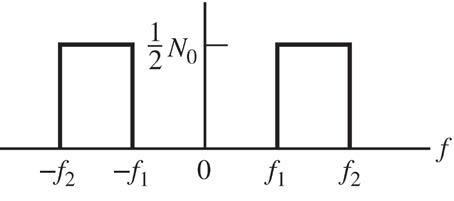
\includegraphics[width=.5\textwidth]{Figure1.jpg}
        \caption{$S_n(f)$}\label{figure1}
    \end{figure}
\end{prob}
\begin{sol}
    
\end{sol}
\end{document}